%%%%%%%%%%%%%%%%%%%%%%%%%%%%%%%%%%%%%%%%%%%%%%%%%%%%%%%%%%%
\section{Умножение вектора на число}
%%%%%%%%%%%%%%%%%%%%%%%%%%%%%%%%%%%%%%%%%%%%%%%%%%%%%%%%%%%
\textbf{Произведением} ненулевого вектора $\vv{a}$ на число $k$
называется такой вектор $\vv{b}$,
длина которого равна $|k|\cdot|\vv{a}|$, причём векторы $\vv{a}$ и $\vv{b}$
сонаправлены при $k\geqslant 0$
и противоположно направлены при $k<0$.

Произведением нулевого вектора на любое число считается нулевой вектор.

\begin{figure}[h]
  \centering
  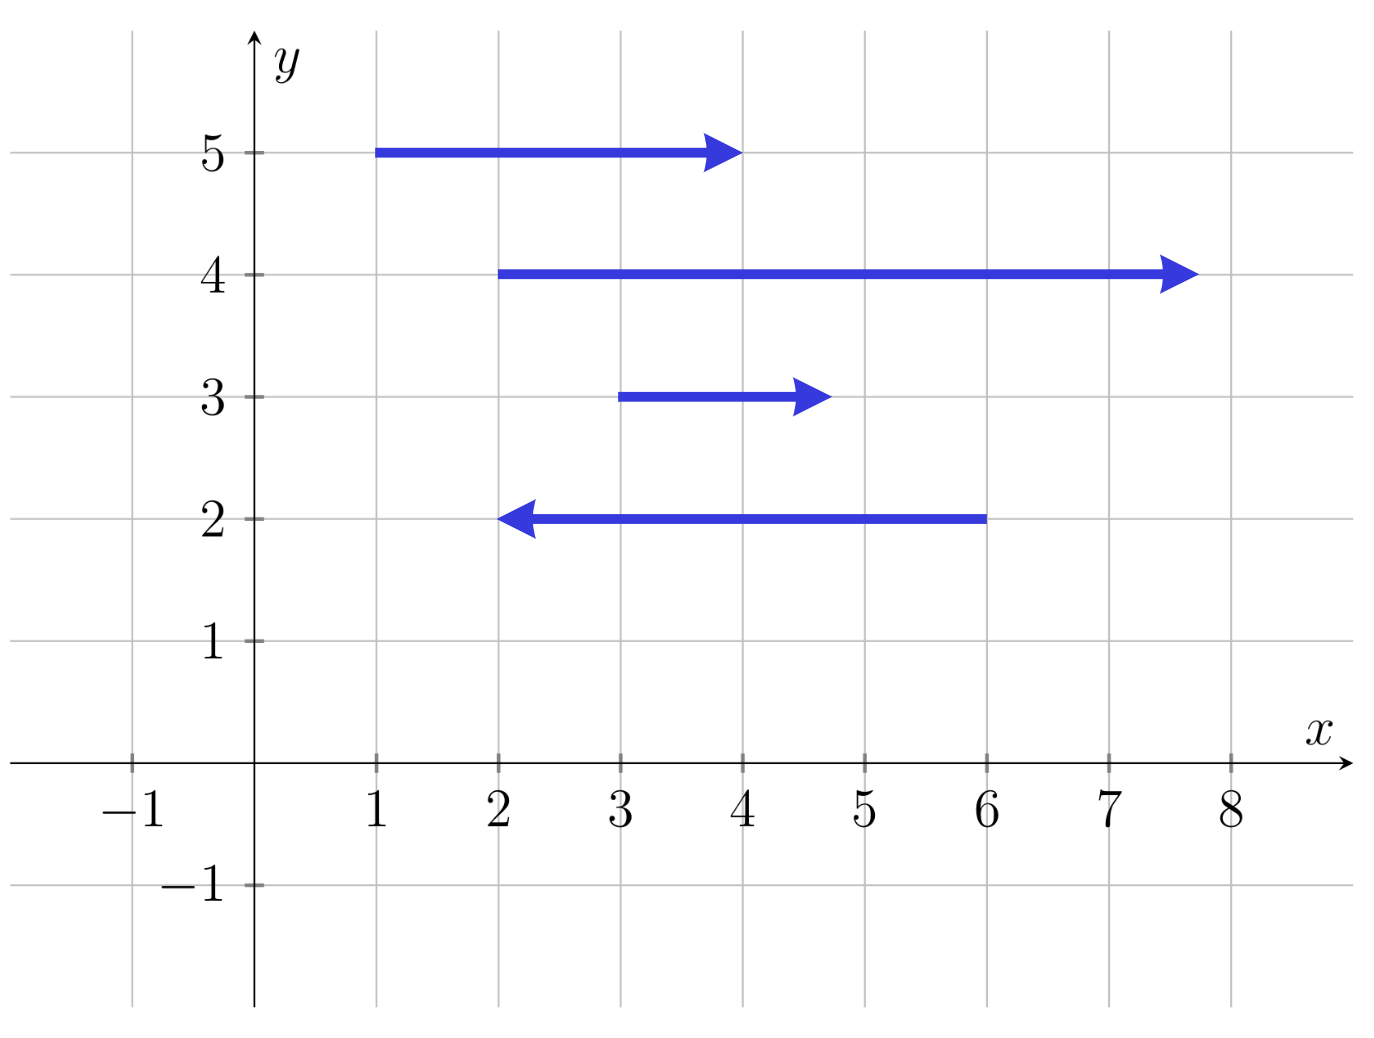
\includegraphics[width=0.7\textwidth]{pics/axis_times.png}
  \put(-210,235){$\vv{a}$}
  \put(-150,202){$\vv{b}$}
  \put(-175,170){$\vv{c}$}
  \put(-185,140){$\vv{d}$}
  \caption{\small Умножение вектора на число.}\label{pic:times}
\end{figure}

На рисунке~\ref{pic:times} изображён вектор $\vv{a}$ и векторы:
\begin{itemize}
\item $\vv{b} = k\cdot \vv{a}$, где $k>1$. В таком случае вектор $\vv{a}$
удлиняется и сохраняет прежнее направление,
\item $\vv{c} = l\cdot \vv{a}$, где $1>l>0$. В этом случае вектор $\vv{a}$ 
укорачивается и также сохраняет прежнее направление,
\item $\vv{d} = m\cdot \vv{a}$, где $m<0$. Вектор $\vv{a}$
меняет направление на противоположное.
\end{itemize}

\clearpage

Приведём \textbf{конкретные примеры}. На рисунке~\ref{pic:times_ex} изображён
вектор $\vv{a}$ длиной 2 клетки (2 единицы измерения отрезков).
А также изображены векторы:
\begin{itemize}
\item $\vv{b} = 2\vv{a}$ (удлинённый в 2 раза вектор $\vv{a}$),
\item $\vv{c} = 1/2\vv{a}$ (укороченный в 2 раза вектор $\vv{a}$),
\item $\vv{d} = -1/2\vv{a}$ (укороченный в 2 раза вектор $\vv{a}$
  и противоположно направленный),
\item $\vv{e} = -\vv{a}$ (равный по модулю вектору $\vv{a}$
  и противоположно направленный),
\item $\vv{f} = -3\vv{a}$ (удлинённый в 3 раза вектор $\vv{a}$
  и противоположно направленный).
\end{itemize}

\begin{figure}[ht]
  \centering
  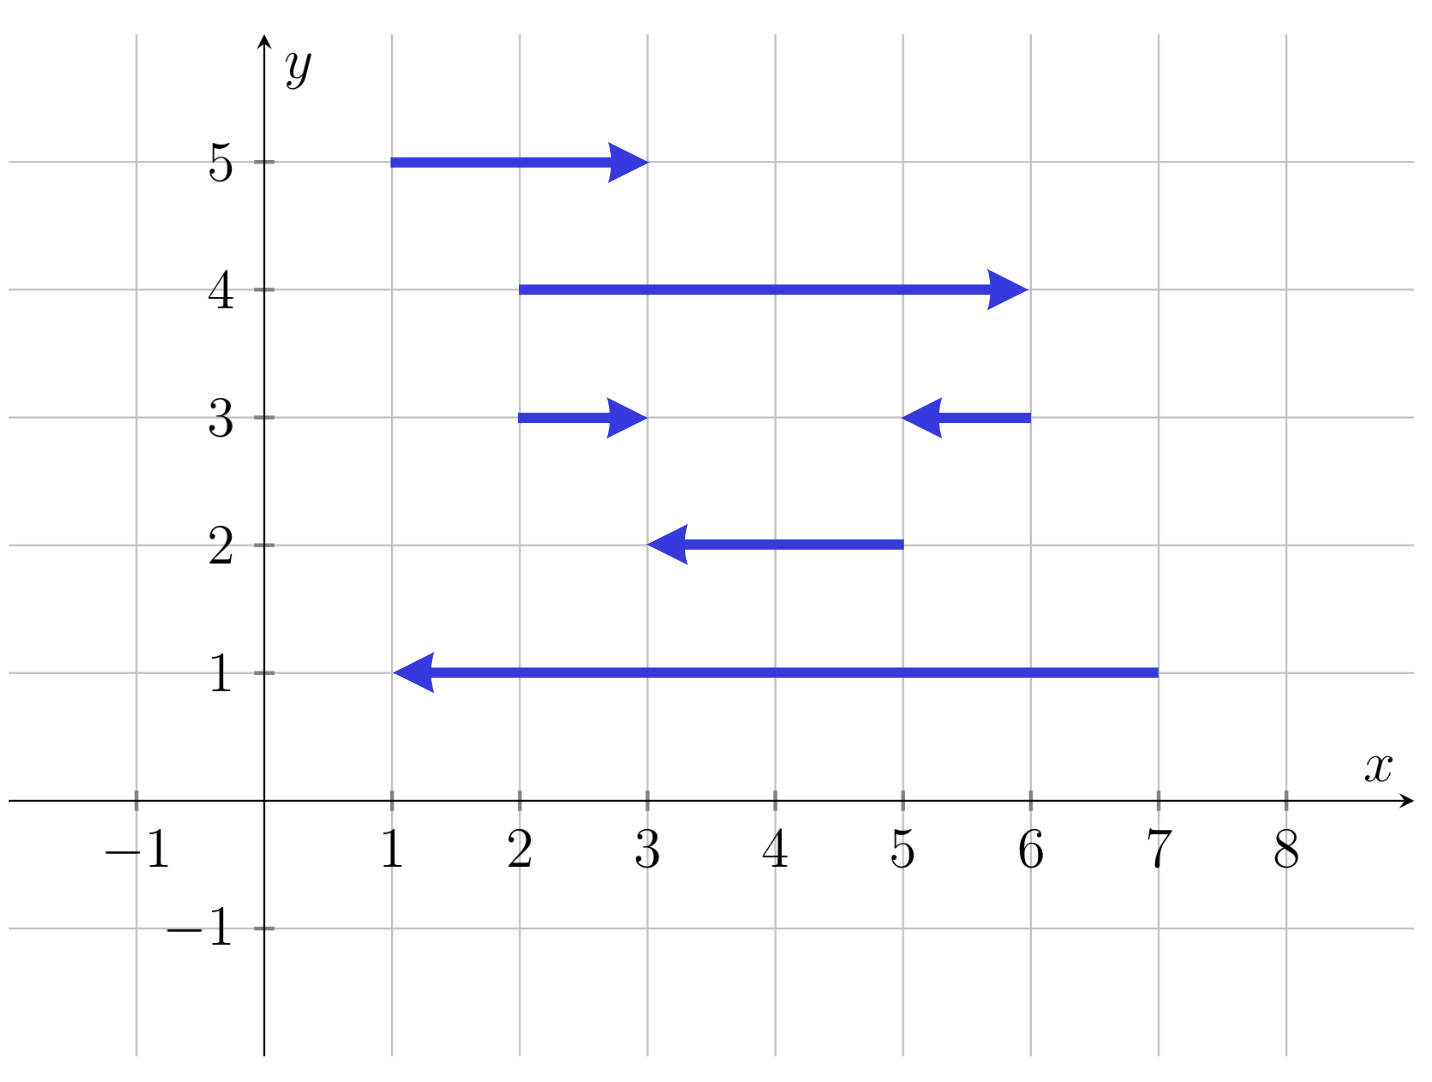
\includegraphics[width=0.7\textwidth]{pics/axis_times_ex.png}
  \put(-230,233){$\vv{a}$}
  \put(-180,203){$\vv{b} = 2\vv{a}$}
  \put(-240,170){$\vv{c} = 1/2\vv{a}$}
  \put(-140,170){$\vv{d} = -1/2\vv{a}$}
  \put(-180,140){$\vv{e} = -\vv{a}$}
  \put(-220,110){$\vv{f} = -3\vv{a}$}
  \caption{\small Умножение вектора на число, примеры.}\label{pic:times_ex}
\end{figure}


